\section{Radar Stick Usage in A/G Aiming Mode}
In A/G aiming mode (AKAN, ARAK, m/71, Rb 75), the target waypoint position is shown as a small circle in the HUD which goes away when unsafing. The waypoint is shown at altitude 0 (for whatever altitude the HUD is showing), so check your altimeter setting if you want it to be useful.

The radar stick in the real AJS has a two stage trigger. Positions are:
\begin{itemize}[nosep]
  \item T0 (released)
  \item T1 (1st stage)
  \item TV (fully pressed)
\end{itemize}

The general idea is that whenever the cursor is used, the pilot holds T1. TV actually 'clicks'. Therefore:
\begin{itemize}[nosep]
  \item for target fix, holding T1 enters fix mode, releasing it cancels, pressing to TV selects new position.
  \item for Rb75, holding T1 allows to move the seeker, releasing it recenters, pressing to TV locks (you can then release).
  \item When lock, do T0 -> T1 -> T0 to unlock).
\end{itemize}

To control all of that in the FlightGear Viggen:
\begin{itemize}[nosep]
  \item \keys{O} is T1
  \item \keys{\shift+O} toggles holding T1
  \item \keys{L} is TV
\end{itemize}

For joysticks:
\begin{itemize}[nosep]
  \item \begin{alltt}/controls/displays/cursor-click-stage1\end{alltt} for T1
  \item \begin{alltt}/controls/displays/cursor-click\end{alltt} for TV
\end{itemize}

\section{AKAN and ARAK}
The m/55 AKAN cannon pods and m/70 ARAK rocket pods share
the same sighting mechanisms and firing procedures.

The m/55 AKAN is a 30mm ADEN cannon pod, with 150 rounds.
Two can be carried on the main wing pylons.

The m/70 ARAK consists of six 135mm rockets, which are all fired in a 0.6 seconds salvo.
Four pods can be carried on the main wing and fuselage pylons.

\subsection{Ranging}
The AJS combines two methods to compute the distance to the target
(i.e.\ the point on which the aiming reticle is located).

\paragraph{Ranging by Triangulation}
Triangulation computes the distance to the target based on aircraft altitude
and the angle between the aiming reticle and the horizon.
Ranging by triangulation assumes that the target altitude is 0,
thus it is essential to properly calibrate indicated altitude by
1.\ setting the altimeter to the target QFE,
or 2.\ using radar-altimeter corrected altitude (switch HÖJD CI SI in position RHM).

Ranging by triangulation is only available if the aiming reticle is at
least 5\textdegree{} below the horizon.

\paragraph{Radar Ranging}
The aircraft main radar is used to compute the range to the ground.
Radar ranging is only used when the following conditions are met.
\begin{itemize}[nosep]
  \item Triangulation ranging is active, and computed distance is at most 7km.
  \item Main mode selector is ANF/CBT.
  \item Roll angle is less than 45\textdegree{}, or trigger safety is open.
\end{itemize}

\paragraph{Remarks}
Because triangulation ranging is required before radar ranging can be enabled,
it is essential to at least approximately calibrate the altimeter.

If triangulation ranging is unavailable (reticle is less than 5\textdegree{} below the horizon)
a fixed distance of 1400m is used to compute reticle position.

\subsection{HUD Aiming Mode}
\begin{figure}[!ht]
  \centering
  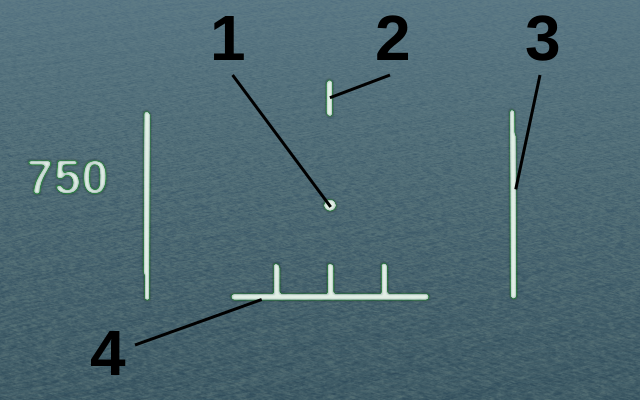
\includegraphics[width=0.45\textwidth]{images/displays/ajs-hud-aiming1.png}
  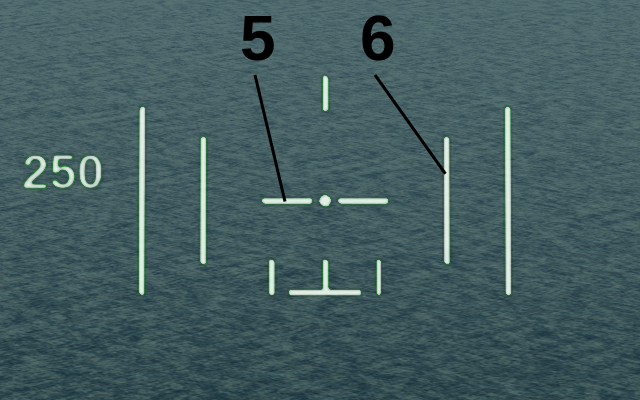
\includegraphics[width=0.45\textwidth]{images/displays/ajs-hud-aiming2.png}

  \begin{multicols}{2}
    \begin{enumerate}[nosep]
      \item \label{item:reticle} Aiming reticle
      \item \label{item:rdr-range} Radar ranging mark.
      \item Side bars, no functionality.
      \item \label{item:distline} Distance line.
      \item \label{item:fire-mark} Firing command lines.
      \item \label{item:pullup-bars} Evasion warning bars.
    \end{enumerate}
  \end{multicols}
  \caption{HUD aiming mode}
  \label{fig:hud-aiming}
\end{figure}

When AKAN or ARAK are selected, the HUD aiming mode (\cref{fig:hud-aiming})
is enabled by switching to mode ANF/CBT, or arming the weapon (trigger unsafe) in mode NAV.

It comports an aiming reticle (\figref{fig:hud-aiming}{item:reticle}),
the digital altitude indicator, and a number of indicators and cues for target range,
which appear in the following order:
\begin{enumerate}
  \item The distance line (\figref{fig:hud-aiming}{item:distline})
    indicates range to the target up to 8km when triangulation ranging is active.
    The side marks indicate the computed firing distance
    (minimum firing distance giving sufficient time for safe evasion).
  \item When radar ranging is active, a vertical bar is displayed above the reticle
    (\figref{fig:hud-aiming}{item:rdr-range}).
  \item 2 seconds before computed firing distance, the distance line blinks.
  \item 0.5 seconds before computed firing distance, the firing command lines appear
    (\figref{fig:hud-aiming}{item:fire-mark}).
  \item When the minimum distance for safe evasion is passed,
    the evasion warning bars start blinking (\figref{fig:hud-aiming}{item:pullup-bars}).
    This indicates that the attack run should be aborted immediately.
\end{enumerate}

Minimum distance for safe evasion is computed to keep the aircraft out of the
explosion debris zone, and assumes a 5g pull, with some margin.

The position of the aiming reticle is correct starting 3 seconds before computed firing distance.
The aiming reticle includes wind compensation.


\section{Rb 75}
The Rb 75 is a Swedish version of the AGM-65A television-guided missile.
It is designed for use against ground targets.
The pilot locks on the target by manually slewing the Rb 75 seeker head using the radar stick.

In the real Viggen, the EP-13 screen to the right of the HUD displayed the Rb
75 seeker image, and was used to lock on the target.

In FlightGear, the EP-13 screen is not functional.
Instead, the seeker position is displayed as a small circle on the HUD.
The seeker is controlled with the radar stick (see \cref{sec:cursor}).
When the seeker is over the target, it can be locked using the radar stick click/select.

\section{Rb 05A}
The Rb 05A is a remote-controlled missile.
It is primarily intended for use against ground and naval targets,
but can also be used against slow-manoeuvring air targets thanks to a proximity fuse.
The missile is guided visually by the pilot.
A flare at the back of the missile helps the pilot to keep sight of it (\cref{fig:rb05-flare}).

\begin{figure}
  \centering
  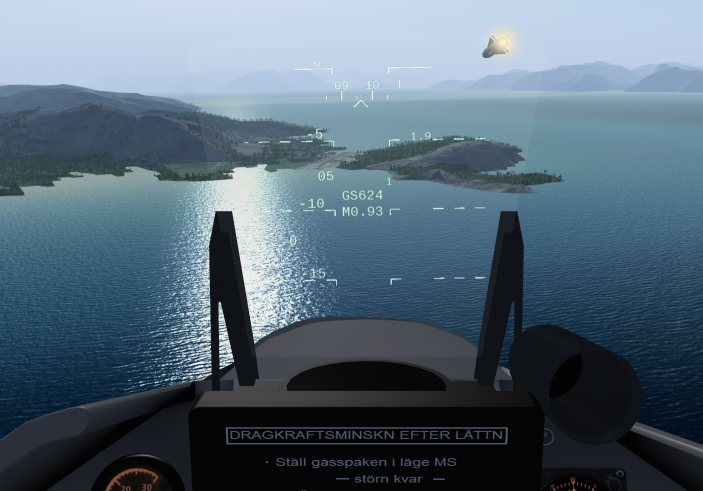
\includegraphics[height=0.3\textwidth]{images/weapons/rb_05a_start_popup.png}
  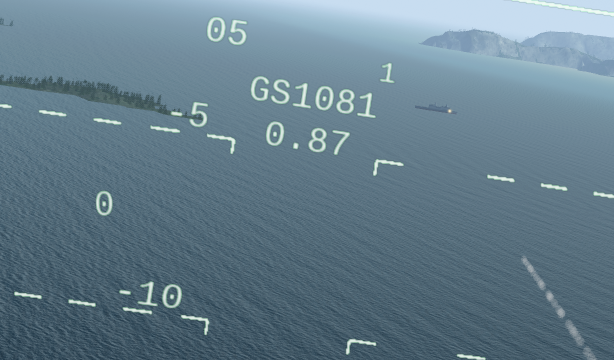
\includegraphics[height=0.3\textwidth]{images/weapons/rb_05a_before_impact_ship.png}
  \caption[Rb 05A flare for visual guidance]{Rb 05A flare for visual guidance.
    On the left, the missile is entering the pilot's field of view just after launch.
    On the right, the missile is about to hit the target ship,
    and the missile flare is visible over the ship
  }
  \label{fig:rb05-flare}
\end{figure}

In FlightGear, the Rb 05A uses the same controls as the radar stick, cf.\ \cref{sec:cursor}.\footnote{%
  In the real Viggen, a separate control stick on the right console was used.
}

\subsection{Procedure}
\begin{enumerate}
  \item Main mode selector to ANF/CBT.
    (\figref{fig:left-panel}{item:main-mode}, shortcuts \keys{M}/\keys{\shift+M}).
  \item Select the Rb 05A (cycle weapons with \keys{C}).
  \item Once in firing position, consider engaging autopilot in ATT or HÖJD/ALT mode to reduce pilot workload.
  \item Identify the target visually.
  \item Unsafe the trigger and fire within 9km of the target.
  \item After 1.7s, missile controls are enabled
    (cf.\ \cref{sec:cursor} for control methods).
    At this point, it should be well within the pilot field of view.
  \item When the missile hits, take evasive manoeuvres, secure the trigger, and switch to NAV mode.
\end{enumerate}

Remarks.
\begin{itemize}
  \item Recommended speed is 700-1150 km/h.
  \item Recommended attitude is a level flight or slight dive,
    so as to not loose sight of the target and the missile.
  \item Recommended altitude is 300-400 meters above ground.
  \item The target do not need to be directly in front of the aircraft
    as the missile can be guided considerably to the side.
    However, doing so makes it harder to aim the missile, and reduces effective range.
  \item The missile flies for ca.\ 24 seconds, giving it a maximum effective range of ca.\ 9 km.
  \item It is easiest to aim the missile using the collimation principle:
    try to keep the missile flare covering the target at all time.
\end{itemize}

\section{Rb-04E and Rb-15F}
These sea target missiles are fire and forget without locking on a target by the pilot. The missiles will find their way to a target somewhat in the direction of the nose at release point. Currently, it is not modelled that the missiles follow waypoints.

The range for the Rb-04E is between 12 and 24 km \textasciimacron for the Rb-15F around 70 km.

To make sure that the missiles doe not splash into the ocean after release:
\begin{itemize}
  \item The launch speed should be around M0.9 (which also makes sure that the missiles reach the max range).
  \item Drop altitude should be above 50 metres - but not above many hundred metres. I.e. you need to pop-up somewhat.
\end{itemize}
